\subsubsection{\stid{2.11} Argobots: Flexible, High-Performance Lightweight Threading }

\paragraph{Overview}

Efficiently supporting massive on-node parallelism demands highly
flexible and lightweight threading and tasking runtimes. At the
same time, existing lightweight abstractions have shortcomings while
delivering generality and specialization.  Our group at Argonne
developed a lightweight, low-level threading and tasking framework,
called Argobots.  The key focus areas of this project are: (1) To
provide a framework that offers powerful capabilities for users to
allow efficient translation of high-level abstractions to low-level
implementations. (2) To provide interoperability with other
programming systems such as OpenMP and MPI as well as with other
software components (e.g., I/O services). (3) To provide a programming
framework that manages hardware resources more efficiently and reduce
interference with co-located applications.

\paragraph{Key Challenges}

Several user-level threading and tasking models have been proposed in
the past to address the shortcomings of OS-level threads, primarily
with respect to cost and flexibility. Their lightweight nature and
flexible generic interface play an important role at managing
efficiently the massive concurrency expected at the Exascale level.
Existing user-level threading and tasking models, however, are either
too specific to applications or architectures or are not powerful or
flexible. Existing runtimes tailored for generic use \cite{GNUPth,
PLDI97_Taura, COSET05_Thibault, COB14_Nakashima, MTAAP08_Wheeler,
PPoPP99_Taura, SenSys06_Dunkels, TBB1, EuroPar08_Perache} are suitable
as common frameworks to facilitate portability and interoperability
but offer insufficient flexibility to efficiently capture higher-level
abstractions, while specialized runtimes \cite{ATC02_Adya,
SolarisThreads, SOSP03_von_Behren, StateThreads, PLDI07_Li,
MTAAP09_Porterfield, WMPP05_Cuvillo, IntelOMP, Nanos++, LCPC96_Kale,
PACT14_Treichler} are tailored to specific environment.

\paragraph{Solution Strategy}

Argobots offers a carefully designed execution model that balances
generality of functionality with providing a rich set of controls to
allow specialization by end users or high-level programming models
\cite{seo2018}.  Delivering high performance in Argobots while
providing a rich set of capabilities is achieved by heavily optimizing
critical paths as well as by exposing configuration knobs and a rich
API, which allow users to trim unnecessary costs. Furthermore,
Argobots honors high degrees of expressibility through the following
three key aspects:

\begin{enumerate}

\item Capturing the requirements of different \emph{work units}, which
are the most basic manageable entities. Work units that require
private stacks and context-saving capabilities, referred to as
\textit{user-level threads} (ULTs, also called \textit{coroutines} or
\textit{fibers}), are fully fledged threads usable in any context.
\emph{Tasklets} do not require private stacks. They are more
lightweight than ULTs because they do not incur context saving and
stack management overheads.  Tasklets, however, are restrictive; they
can be executed only as atomic work units that run to completion
without context switching.

\item Exposing hardware computational units through \emph{execution
streams} (ESs) as OS-level threads to execute work units. Unlike
existing generic runtimes, ESs are exposed to and manageable by users.

\item Allowing full control over \emph{work unit management}.  Users
can freely manage \emph{scheduling} and mapping of work units to ESs
through \emph{thread pool} management, and thus achieving the desired
behavior. Figure~\ref{fig:sollve-argobots} illustrates the various
building blocks in the Argobots framework and the interactions between
them to build a hypothetical system.

\end{enumerate}

\begin{figure}[htb]
  \centering
  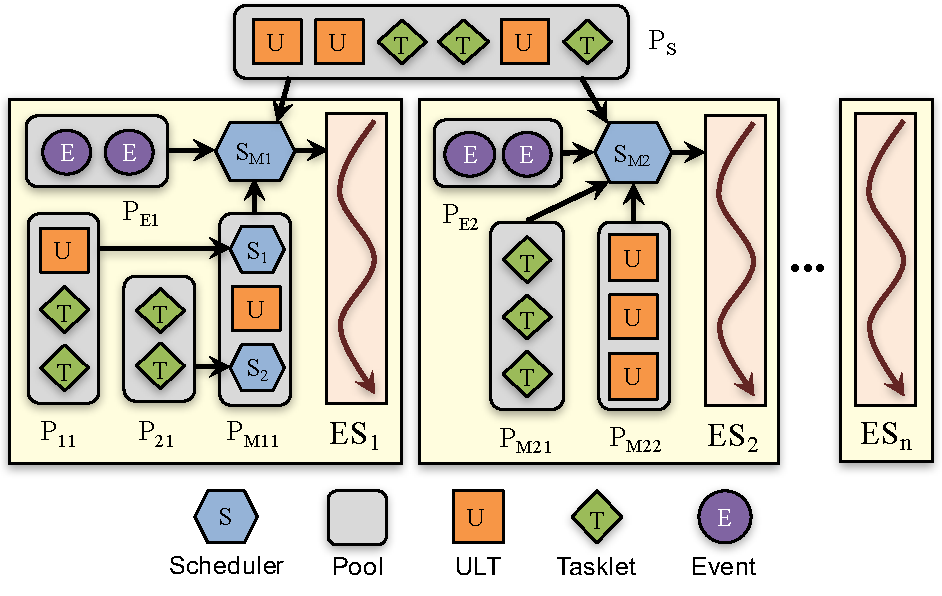
\includegraphics[height=3in]{projects/2.3.2-Tools/2.3.2.11-SOLLVE/SOLLVE-ARGOBOTS.pdf}
  \caption{\label{fig:sollve-argobots}Argobots execution model}
\end{figure}

\paragraph{Recent Progress}

Threading overheads are crucial for fine-grained parallel applications
and runtimes running in massively parallel environments.  We have
found that the timing of yield operations highly affects the
performance of lightweight threads~\cite{iwasaki2018}, but other
factors remained unexplored.  We further optimized fork-join overheads
by exploring new threading methods with respect to stack allocation
timing and scheduling policies and a wider range of modern hardware
architectures.  Our evaluation shows that our child-first scheduling
yields promising results for deep and narrow recursive task-parallel
programs while the parent-first scheduling is good for flat
parallelism.  Our study helps users and application developers choose
the best threading methods that fit their hardware architectures and
application workloads and maximize the scalability~\cite{iwasaki2020}.

Integration with other runtime systems is fundamentally important for
the Argobots project.  BOLT, a SOLLVE OpenMP runtime over
Argobots~\cite{BOLT}, is one of the most successful parallel
programming systems using Argobots.  Our enhancements of Argobots
threads lowers the cost of OpenMP threading and tasking.  The Argobots
project continues to improve interoperability with communication
layers such as MPI runtimes (e.g., MPICH and Open~MPI) and Margo, a
Mercury RPC over Argobots.  To help their performance analysis, our
latest Argobots 1.1a1 release includes a lightweight yet powerful
profiling interface, which helps runtime developers pinpointing a
performance problem in these systems.  I/O service is one of the most
important application areas for Argobots. Intel DAOS, a next-
generation high-performance storage system developed by Intel, uses
Argobots to efficiently handle asynchronous I/O messages.  We are
working together to improve Argobots by providing a better debugging
interface such as stack dump features. Our CI testing has been
extended for various CPU architectures, operating systems, and
compilers to cover most of the DOE HPC platforms.  Thanks to our CI,
Argobots 1.1a1 works on major UNIX-based platforms including Ubuntu,
FreeBSD, CentOS, macOS, and Solaris. Argobots supports most CPU
architectures with special optimizations for Intel/AMD x86/64,
ARMv8-A, and POWER 8 and 9. Argobots can be compiled with numerous C
compilers including GCC, Clang, ICC (Intel), XLC (IBM), PGCC (PGI),
Solaris Studio (Oracle), and Arm C Compiler for HPC (ARM).

The innovative design and implementation of Argobots are highly
recognized.  Argobots was named a finalist for the 2020 R\&D 100
Awards.  The prestigious R\&D 100 competition, sponsored by R\&D
Magazine, recognizes the 100 most innovative technologies of the
previous year.  Argobots, a lightweight and highly flexible
multithreading framework, was chosen as a finalist for the 2020 R\&D
100 Awards.

\paragraph{Next Steps}

Argobots continues to implement new features and optimizations for
application needs, while our substantial efforts will be made to
promote integration and composition with other systems. Our major
ongoing and planned steps are as follows.

\begin{enumerate}

\item Further integration with other applications and runtimes
including MPI runtimes including MPICH and Open MPI.  In collaboration
with MPICH and Open MPI developers, we will further optimize their
Argobots interoperability layers by utilizing user-level threading
techniques.

\item Enhanced interoperability of multiple components that are not
aware of Argobots.  Unfortunately, not all applications are written
for lightweight ULTs; some programs suffer from core starvation and,
in the worst case, deadlocks if they are running on Argobots.  To
address this issue, we are investigating an approach that is as
lightweight as the current Argobots ULTs while it has the OS-implicit
preemption functionality that traditional OS-level threads have.

\end{enumerate}
